\documentclass[aspectratio=169,11pt]{beamer}
\usepackage[T1]{fontenc}
\usepackage{lmodern,amsmath,amssymb,mathtools,bm,booktabs,array,graphicx,tikz}
\usetikzlibrary{arrows.meta,positioning,calc,decorations.pathreplacing,patterns}
\definecolor{ink}{HTML}{17344D}\definecolor{accent}{HTML}{087E8B}\definecolor{pale}{HTML}{EDF5F5}\definecolor{gold}{HTML}{AD6B19}
\providecommand{\dd}{\,\mathrm{d}}\providecommand{\R}{\mathbb{R}}
\providecommand{\E}{\mathbb{E}}\providecommand{\Var}{\operatorname{Var}}
\providecommand{\Cov}{\operatorname{Cov}}\providecommand{\diag}{\operatorname{diag}}
\providecommand{\norm}[1]{\left\lVert#1\right\rVert}
\providecommand{\abs}[1]{\left|#1\right|}
\usefonttheme{professionalfonts}
\setbeamercolor{normal text}{fg=black,bg=white}
\setbeamercolor{frametitle}{fg=ink,bg=white}
\setbeamercolor{title}{fg=ink}\setbeamercolor{structure}{fg=accent}
\setbeamercolor{block title}{fg=ink,bg=pale}\setbeamercolor{block body}{fg=black,bg=pale!40}
\setbeamercolor{alerted text}{fg=accent}
\setbeamerfont{frametitle}{size=\Large,series=\bfseries}
\setbeamerfont{title}{size=\LARGE,series=\bfseries}
\setbeamertemplate{navigation symbols}{}
\setbeamersize{text margin left=.7cm,text margin right=.7cm}
\setbeamertemplate{frametitle}{\vspace{.18cm}\insertframetitle\par\vspace{.1cm}{\color{accent}\hrule height .6pt}\vspace{.12cm}}
\newcommand{\notestarget}{notes.pdf}\newcommand{\noteslabel}{Notes}
\setbeamertemplate{footline}{\hspace{.7cm}\color{ink}\scriptsize Mathematical Modeling\quad\href{\notestarget}{\noteslabel}\hfill\insertframenumber\,/\,\inserttotalframenumber\hspace{.7cm}\vspace{.18cm}}
\setbeamercovered{invisible}
\hypersetup{pdfauthor={Zan Ahmad},pdftitle={Resistance networks: constitutive laws, pressure, and conservation},pdfpagemode=UseNone}
\begin{document}
\begin{frame}[plain]\vfill
{\small\color{accent} Mathematical Modeling \quad Lecture 2}\par\medskip
{\raggedright\hyphenpenalty=10000\exhyphenpenalty=10000\LARGE\bfseries\color{ink} Resistance networks: constitutive laws, pressure, and conservation}\par\bigskip
Zan Ahmad\par\smallskip
{\small Fall 2024}\par\vfill\end{frame}
\renewcommand{\notestarget}{notes.pdf\#note-linear-resistance-is-a-local-constitutive-assumption}
\begin{frame}[t,fragile,label=slide-conservation-needs-a-constitutive-law]{Conservation needs a constitutive law}
At a non-storing node, inflow equals outflow.\pause{}\[Q_{i\to j}=\frac{P_i-P_j}{R_{ij}}=G_{ij}(P_i-P_j).\]The first statement connects links; the second describes one link.
\end{frame}
\renewcommand{\notestarget}{notes.pdf\#note-linear-resistance-is-a-local-constitutive-assumption}
\begin{frame}[t,fragile,label=slide-choose-an-orientation-once]{Choose an orientation once}
\[Q_{A\to B}=G(P_A-P_B),\qquad Q_{B\to A}=-Q_{A\to B}.\]\pause{} If $P_B>P_A$, the first variable is negative. A reference arrow is not an ideal valve.
\end{frame}
\renewcommand{\notestarget}{notes.pdf\#note-linear-resistance-is-a-local-constitutive-assumption}
\begin{frame}[t,fragile,label=slide-dimensions-and-dissipation]{Dimensions and dissipation}
\[[R]=\frac{\mathrm{mmHg}\,\mathrm{min}}{\mathrm L},\qquad[G]=\frac{\mathrm L}{\mathrm{min}\,\mathrm{mmHg}}.\]\pause{}\[(P_i-P_j)Q_{i\to j}=R_{ij}Q_{i\to j}^{2}\geq0.\]
\end{frame}
\renewcommand{\notestarget}{notes.pdf\#note-boundary-pressures-are-data-interior-pressures-are-unknowns}
\begin{frame}[label=slide-prescribed-endpoints-and-unknown-interiors-figure]{Prescribed endpoints and unknown interiors}
\centering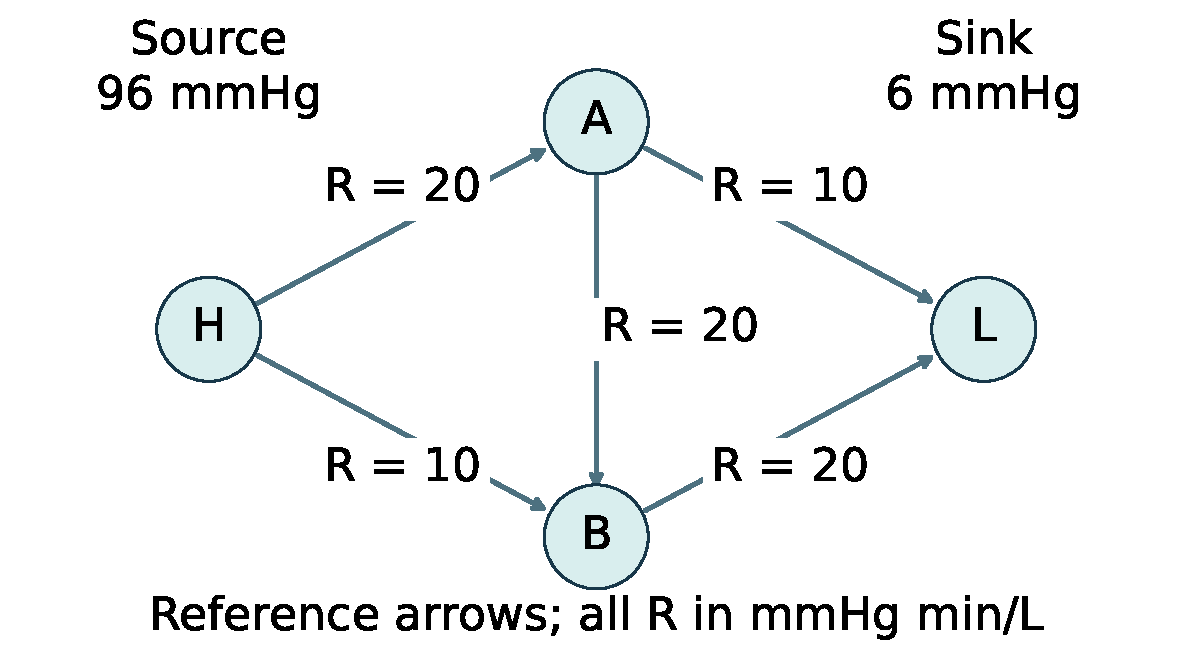
\includegraphics[width=.98\linewidth,height=.69\textheight,keepaspectratio]{presentation-figures/network.pdf}\end{frame}
\renewcommand{\notestarget}{notes.pdf\#note-boundary-pressures-are-data-interior-pressures-are-unknowns}
\begin{frame}[t,fragile,label=slide-prescribed-endpoints-and-unknown-interiors]{Prescribed endpoints and unknown interiors}
$P_H=96$, $P_L=6$ mmHg; solve for $P_A,P_B$.\pause{}\[R_{HA}=20,\ R_{AL}=10,\ R_{HB}=10,\ R_{BL}=20,\ R_{AB}=20.\]Every link is open and has positive resistance.
\end{frame}
\renewcommand{\notestarget}{notes.pdf\#note-boundary-pressures-are-data-interior-pressures-are-unknowns}
\begin{frame}[t,fragile,label=slide-write-the-a-balance]{Write the A balance}
\[\underbrace{\frac{96-P_A}{20}}_{H\to A}-\underbrace{\frac{P_A-6}{10}}_{A\to L}-\underbrace{\frac{P_A-P_B}{20}}_{A\to B}=0.\]\pause{} Each term is a flow in L/min.
\end{frame}
\renewcommand{\notestarget}{notes.pdf\#note-boundary-pressures-are-data-interior-pressures-are-unknowns}
\begin{frame}[t,fragile,label=slide-write-the-b-balance]{Write the B balance}
\[\frac{96-P_B}{10}+\frac{P_A-P_B}{20}-\frac{P_B-6}{20}=0.\]\pause{} The bridge term has the opposite sign from its appearance at A.
\end{frame}
\renewcommand{\notestarget}{notes.pdf\#note-solve-the-two-unknowns-then-recover-every-flow}
\begin{frame}[t,fragile,label=slide-collect-and-eliminate]{Collect and eliminate}
\[4P_A-P_B=108,\qquad-P_A+4P_B=198.\]\pause{}\[15P_A=630\quad\Rightarrow\quad P_A=42,\ P_B=60\ \mathrm{mmHg}.\]
\end{frame}
\renewcommand{\notestarget}{notes.pdf\#note-solve-the-two-unknowns-then-recover-every-flow}
\begin{frame}[label=slide-recover-five-signed-flows-figure]{Recover five signed flows}
\centering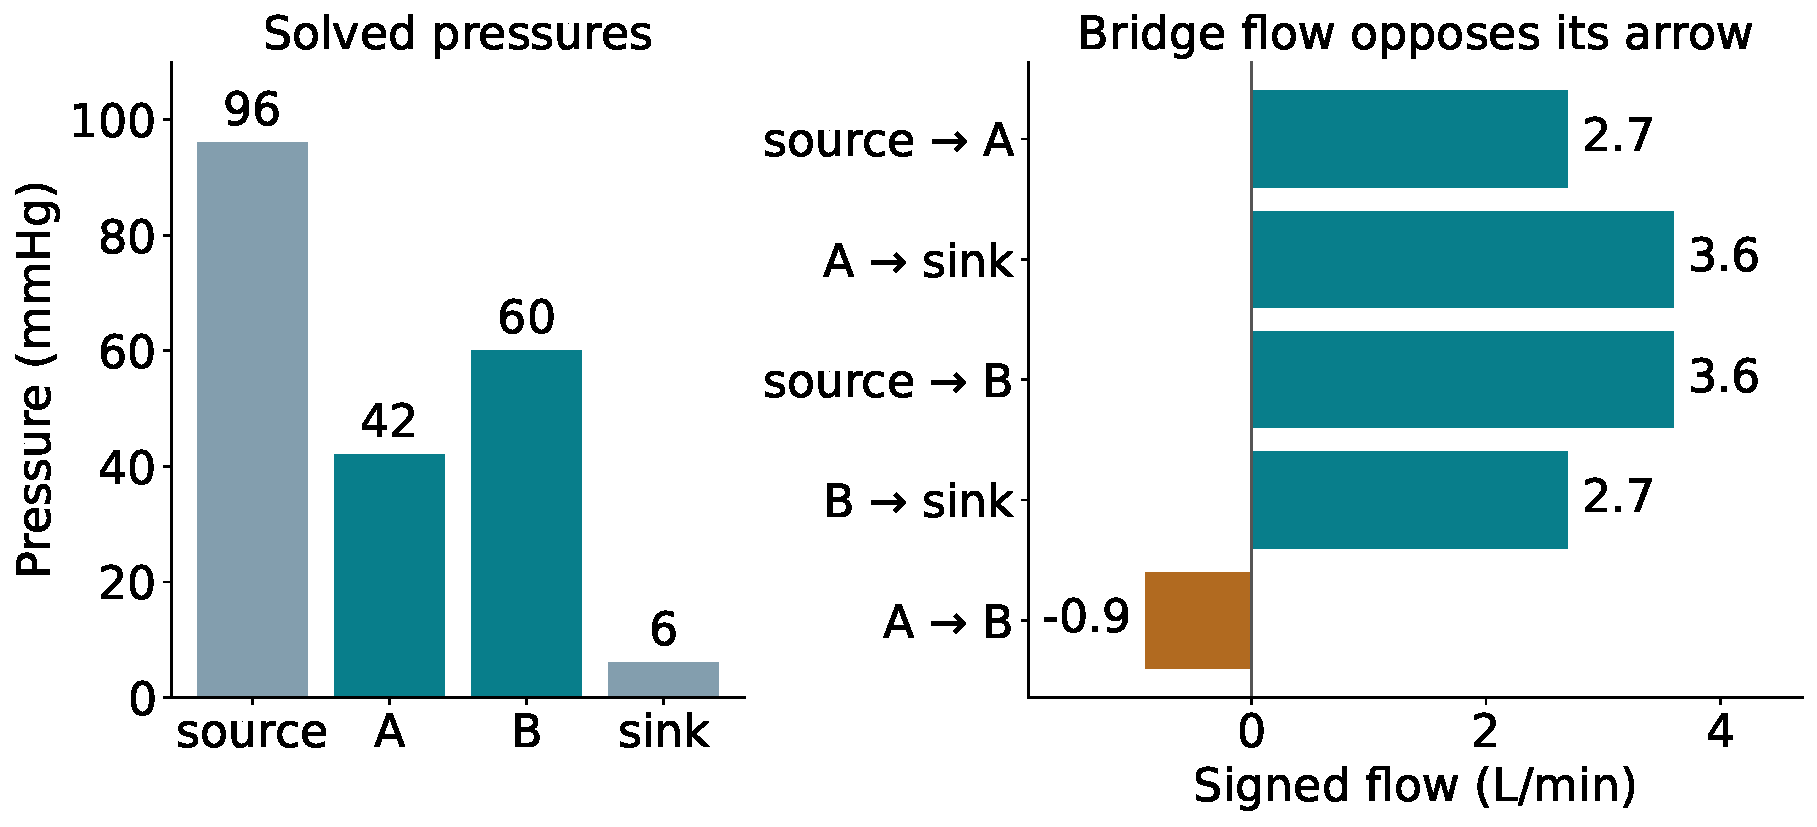
\includegraphics[width=.98\linewidth,height=.69\textheight,keepaspectratio]{presentation-figures/pressures-and-flows.pdf}\end{frame}
\renewcommand{\notestarget}{notes.pdf\#note-solve-the-two-unknowns-then-recover-every-flow}
\begin{frame}[t,fragile,label=slide-recover-five-signed-flows]{Recover five signed flows}
\[Q_{HA}=2.7,\ Q_{AL}=3.6,\ Q_{HB}=3.6,\ Q_{BL}=2.7,\]\[Q_{AB}=(42-60)/20=-0.9\quad[\mathrm L/\mathrm{min}].\]\pause{} The bridge carries fluid from B to A.
\end{frame}
\renewcommand{\notestarget}{notes.pdf\#note-solve-the-two-unknowns-then-recover-every-flow}
\begin{frame}[t,fragile,label=slide-independent-node-and-boundary-audits]{Independent node and boundary audits}
\[A:\ 2.7-3.6+0.9=0,\qquad B:\ 3.6-0.9-2.7=0.\]\pause{}\[Q_{\rm in}=2.7+3.6=6.3=3.6+2.7=Q_{\rm out}.\]
\end{frame}
\renewcommand{\notestarget}{notes.pdf\#note-the-conductance-matrix-and-a-uniqueness-argument}
\begin{frame}[t,fragile,label=slide-the-graph-matrix]{The graph matrix}
\[\sum_jG_{ij}(P_i-P_j)=0\quad\Longrightarrow\quad L_{II}\mathbf p=\mathbf b.\]\pause{}\[L_{II}=\begin{bmatrix}.20&-.05\\-.05&.20\end{bmatrix},\qquad\mathbf b=\begin{bmatrix}5.4\\9.9\end{bmatrix}.\]
\end{frame}
\renewcommand{\notestarget}{notes.pdf\#note-the-conductance-matrix-and-a-uniqueness-argument}
\begin{frame}[t,fragile,label=slide-why-the-solution-is-unique]{Why the solution is unique}
Let $z=0$ on prescribed-pressure nodes.\[\mathbf z^TL_{II}\mathbf z=\sum_{\{i,j\}}G_{ij}(z_i-z_j)^2\geq0.\]\pause{} If each interior component reaches a boundary, equality implies $z=0$.
\end{frame}
\renewcommand{\notestarget}{notes.pdf\#note-the-conductance-matrix-and-a-uniqueness-argument}
\begin{frame}[t,fragile,label=slide-an-interior-pressure-is-a-weighted-mean]{An interior pressure is a weighted mean}
\[P_i=\frac{\sum_jG_{ij}P_j}{\sum_jG_{ij}}.\]\pause{} Therefore $6\leq P_i\leq96$ mmHg in this connected passive example. An interior source would change this conclusion.
\end{frame}
\renewcommand{\notestarget}{notes.pdf\#note-transformations-that-expose-errors}
\begin{frame}[t,fragile,label=slide-change-the-pressure-reference]{Change the pressure reference}
\[P_i^{\prime}=P_i+c\quad\Rightarrow\quad P_i^{\prime}-P_j^{\prime}=P_i-P_j.\]\pause{} All flows are unchanged. Shift every endpoint and interior pressure consistently.
\end{frame}
\renewcommand{\notestarget}{notes.pdf\#note-transformations-that-expose-errors}
\begin{frame}[t,fragile,label=slide-scale-every-resistance]{Scale every resistance}
\[R_e^{\prime}=kR_e,\quad G_e^{\prime}=G_e/k.\]\pause{}\[(L_{II}/k)\mathbf p^{\prime}=\mathbf b/k\Rightarrow\mathbf p^{\prime}=\mathbf p,\quad Q_e^{\prime}=Q_e/k.\]
\end{frame}
\renewcommand{\notestarget}{notes.pdf\#note-transformations-that-expose-errors}
\begin{frame}[t,fragile,label=slide-series-and-parallel-follow-from-balances]{Series and parallel follow from balances}
In series, one common $Q$ gives $\Delta P=Q(R_1+R_2)$.\pause{}\par In parallel, one common $\Delta P$ gives $Q_{\rm total}=(G_1+G_2)\Delta P$.\pause{}\[R_{\rm eff}=\frac{90}{6.3}=\frac{100}{7}.\]
\end{frame}
\renewcommand{\notestarget}{notes.pdf\#note-computational-residuals-and-the-scope-of-a-claim}
\begin{frame}[t,fragile,label=slide-a-numerical-residual-is-necessary]{A numerical residual is necessary}
\[\mathbf r=L_{II}\mathbf p-\mathbf b.\]\pause{} Solve the matrix system, then recover flows. Add reference-shift and resistance-scaling tests; do not use an inverse as an intermediate numerical object.
\end{frame}
\renewcommand{\notestarget}{notes.pdf\#note-computational-residuals-and-the-scope-of-a-claim}
\begin{frame}[t,fragile,label=slide-dynamic-extensions-storage-valves-and-pumping]{Dynamic extensions: storage, valves, and pumping}
Storage introduces $\dot V_i$, a valve restricts direction, and active contraction changes a pressure--volume relation.\pause{}\par Each mechanism changes a specific equation. None is supplied by the present steady resistor solve.
\end{frame}
\end{document}
